\chapter{Knjižnica pandas}

\section{Delo s podatki}

Podatkovne vede \angl{data sciences}, ki se ukvarjajo z manipulacijo in analizo podatkov, so v današnjem času postale nepogrešljive na različnih področjih ne samo znanosti, temveč tudi različnih vej gospodarstva (npr. ciljno oglaševanje, organizacija dela, planiranje procesov) in negospodarstva (npr. zdravstvo in medicina). Podatkovne vede namreč na podlagi zajema in analize (večjih količin) podatkov nudijo podporo procesom odločanja, s čimer lahko razpoložljive vire izkoristimo bolj učinkovito. Kdor zna delati s podatki ima danes službo zagotovljeno, še posebej, če zna ta znanja uporabiti na svojem primarnem strokovnem področju, kot je npr. kemija. 

Če za bolj resno analizo in manipulacijo podatkov uporabljamo programski jezik Python, bomo slej ko prej pristali na uporabi knjižnice pandas \angl{Python Data Analysis Library}, ki predstavlja moderno in hitro orodje za delo z večjimi količinami podatkov. Delo s knjižnico pandas je namreč v današnjem času postalo sinonim za delo z večjimi količinami podatkov v jeziku Python. V sledečem poglavju si bomo pogledali par primerov uporabe knjižnice pandas, ki zgolj nakazujejo prednosti uporabe te knjižnice. 

\section{Knjižnica pandas in \texttt{dataframe}}

Za uporabo moramo knjižnico pandas najprej namestiti z orodjem \texttt{pip}, kar že znamo. V ukazni vrstici svojega operacijskega sistema napišemo:
\begin{lstlisting}[language=bash]
> pip install pandas
\end{lstlisting}
Zdaj lahko knjižnico uvozimo v svoj program oziroma v svoje delovno okolje, ponavadi pod psevdonimom \texttt{pd}:
\begin{lstlisting}[language=python]
>>> import pandas as pd
\end{lstlisting}
Večje količine podatkov bomo ponavadi brali iz datotek zapisanih v obliki CSV. Pandas tako branje omogoča preko funkcije \texttt{read\_csv}. Poskusimo kar na našem zgledu s plačami.
\begin{lstlisting}[language=python]
>>> pd.read_csv('place.csv')
UnicodeDecodeError: 'utf-8' codec can't decode byte
0xe8 in position 6: invalid continuation byte
\end{lstlisting}
Tole ni delovalo, ker moramo podati pravilno dekodiranje. Nastavimo argument \texttt{encoding}, poleg tega pa rezultat branja shranimo v spremenljivko:
\begin{lstlisting}[language=python]
>>> df = pd.read_csv('place.csv', encoding="cp1250")
\end{lstlisting}
Funkcija \texttt{read\_csv} vrača prebrane podatke v obliki strukture \texttt{dataframe}, ki predstavlja tabelo z zapisanimi podatki. Prvih pet vrstic tabele lahko dobimo z metodo \texttt{head()}. Poglejmo kaj smo prebrali.
\begin{lstlisting}[language=python]
>>> df.head()
  Povprečne mesečne bruto in neto plače pri pravnih
  osebah javnega in zasebnega sektorja, Slovenija,
  mesečno
0  MESEC\t"SEKTOR"\t"Bruto plača Plača za mesec[E...                                                        
1          2014M01\t"Javni sektor"\t1758.50\t1151.30                                                        
2         2014M01\t"Zasebni sektor"\t1421.34\t932.14                                                        
3          2014M02\t"Javni sektor"\t1745.63\t1136.41                                                        
4         2014M02\t"Zasebni sektor"\t1406.47\t922.19  
\end{lstlisting}
Tabela še vedno ni \emph{tabela}. Smiselno bi bilo, da prve vrstice z opisom vsebine datoteke, izpustimo (to smo naredili tudi prej), tako da izbirnemu argumentu \texttt{skiprows} priredimo vrednost 2. Zakaj bomo tokrat izpustili 2 vrstici, ko smo datoteko brali z metodo \texttt{read} pa smo izpustili 3? Struktura \texttt{dataframe} bo prvo prebrano vrstico (za izpuščenima dvema vrsticama) uporabila kot glavo tabele. Druga stvar, ki jo moralo našemu bralniku nastaviti je še ločilo oziroma separator, ki je v tem primeru tabulator oziroma znak \texttt{'$\backslash$t'}. Tega nastavimo preko argumenta \texttt{sep}. Poskusimo datoteko še enkrat prebrati:
\begin{lstlisting}[language=python]
>>> df = pd.read_csv('place.csv', 
                     encoding="cp1250", 
                     skiprows=2, 
                     sep='\t')
\end{lstlisting}
Preverimo, katere stolpce imamo v tabeli
\begin{lstlisting}[language=python]
>>> df.columns
Index(['MESEC', 'SEKTOR', 'Bruto plača Plača za
mesec[EUR]', 'Neto plača Plača za mesec[EUR]'],
      dtype='object')
\end{lstlisting}
Na prvi poglej izgleda, da smo tabelo zdaj uspešno uvozili. Stolpce lahko tudi preimenujemo v kaj krajšega:
\begin{lstlisting}[language=python]
>>> df.columns = ['mesec', 'sektor', 'bruto', 'neto']
\end{lstlisting}
Zdaj pa izpišimo prvih pet vrstic tabele:
\begin{lstlisting}[language=python]
>>> df.head()
    mesec   sektor          bruto   neto  
0   2014M01 Javni sektor    1758.50 1151.30
1   2014M01 Zasebni sektor  1421.34 932.14
2   2014M02 Javni sektor    1745.63 1136.41
3   2014M02 Zasebni sektor  1406.47 922.19
4   2014M03 Javni sektor    1741.44 1133.47
\end{lstlisting}
Preverimo lahko tudi strukturo tabele preko atributa \texttt{shape}:
\begin{lstlisting}[language=python]
>>> df.shape
(148, 4)
\end{lstlisting}
Naša tabela ima torej 148 vrstic in 4 stolpce. Do osnovne statistike lahko pridemo preko metode \texttt{describe}
\begin{lstlisting}
>>> df.describe()
             bruto         neto
count   148.000000   148.000000
mean   1694.473919  1099.702230
std     217.336086   133.755268
min    1393.050000   915.740000
25%    1471.885000   963.452500
50%    1743.535000  1136.695000
75%    1865.522500  1203.942500
max    2174.570000  1408.770000
\end{lstlisting}
Ta nam vrne osnovno statistiko, ampak zgolj za numerične stolpce. Težava je le v tem, da imamo zdaj javni in zasebni sektor združena skupaj. Tudi to bomo rešili v kratkem.

\section{Indeksiranje tabel}

Tabele indeksiramo podobno kot sezname, le da tokrat indeksiranje izvajamo po stolpcih. Do stolpca z oznako  \texttt{bruto} bi torej lahko prišli takole:
\begin{lstlisting}[language=python]
>>> df['bruto']
0      1758.50
1      1421.34
2      1745.63
        ...
146    2055.48
147    1682.86
Name: bruto, Length: 148, dtype: float64
\end{lstlisting}
Lahko bi dostopali tudi do več stolpcev naenkrat, tako da pri indeksiranju podamo seznam stolpcev:
\begin{lstlisting}[language=python]
>>> df[['bruto','neto']]
       bruto     neto
0    1758.50  1151.30
1    1421.34   932.14
2    1745.63  1136.41
        ...
146  2055.48  1327.33
147  1682.86  1098.04
[148 rows x 2 columns]
\end{lstlisting}

Kaj pa, če želimo priti do določenih vrstic? V tem primeru uporabimo metodo \texttt{loc}, ki ji znotraj oglatih oklepajev podamo \texttt{index} vrstice. Ko smo prej izpisali tabelo, se je pred stolpcem \texttt{mesec} izpisal dodaten stolpcev \texttt{index}. Ko tabelo preberemo, ima ta stolpcev vrednosti od 0 do števila vrstic $-$ 1, lahko pa \texttt{index} nastavimo tudi na kaj drugega. Do 0-te vrstice bi torej prišli takole:
\begin{lstlisting}[language=python]
>>> df.loc[0]
mesec          2014M01
sektor    Javni sektor
bruto           1758.5
neto            1151.3
Name: 0, dtype: object
\end{lstlisting}
Metodi \texttt{loc} lahko podamo tudi stolpec ali seznam stolpcev:
\begin{lstlisting}[language=python]
>>> df.loc[0,'bruto']
1758.5
\end{lstlisting}
Stolpcev \texttt{index} lahko spremenimo tudi na kakšnega izmed obstoječih stolpcev. Naredimo novo tabelo, ki bo imela za \texttt{index} kar stolpec \texttt{mesec}:
\begin{lstlisting}[language=python]
>>> df2 = df.set_index('mesec')
>>> df2.head()
                 sektor    bruto     neto
mesec                                    
2014M01    Javni sektor  1758.50  1151.30
2014M01  Zasebni sektor  1421.34   932.14
2014M02    Javni sektor  1745.63  1136.41
2014M02  Zasebni sektor  1406.47   922.19
2014M03    Javni sektor  1741.44  1133.47
\end{lstlisting}
Zdaj bi do vrstico metodi \texttt{loc} podali kar mesec, ki nas zanima:
\begin{lstlisting}[language=python]
>>> df2.loc['2018M01']
                 sektor    bruto     neto
mesec                                    
2018M01    Javni sektor  1936.41  1246.69
2018M01  Zasebni sektor  1526.94  997.06
\end{lstlisting}

Zadnji način indeksiranja je z uporabo metode \texttt{iloc}, kateri podamo številko vrstice lahko pa tudi stolpca. Takole:
\begin{lstlisting}[language=python]
>>> df.iloc[1]
mesec            2014M01
sektor    Zasebni sektor
bruto            1421.34
neto              932.14
Name: 1, dtype: object
>>> df.iloc[1,3]
932.14
\end{lstlisting}
Seveda lahko s to metodo delamo tudi rezine. Če nas zanimajo npr vse vrstice, stolpca številka 2, bi to napisali takole:
\begin{lstlisting}[language=python]
>>> df.iloc[:,2]
0      1758.50
1      1421.34
2      1745.63
        ...
146    2055.48
147    1682.86
Name: bruto, Length: 148, dtype: float64
\end{lstlisting}

\section{Filtriranje podatkov}
Podatke lahko filtriramo na podoben način kot pri uporabi strukture \texttt{ndarray}. Lahko bi npr. pogledali samo tiste vrstice, ki pripadajo javnemu sektorju:
\begin{lstlisting}[language=python]
>>> df['sektor'] == 'Javni sektor'
0       True
1      False
2       True
        ...
146     True
147    False
Name: sektor, Length: 148, dtype: bool
\end{lstlisting}
Tako dobljen rezultat primerjanja lahko zdaj uporabimo pri indeksiranju:
\begin{lstlisting}[language=python]
>>> df[df['sektor'] == 'Javni sektor']
mesec        sektor    bruto     neto
0    2014M01  Javni sektor  1758.50  1151.30
2    2014M02  Javni sektor  1745.63  1136.41
4    2014M03  Javni sektor  1741.44  1133.47
        ...
144  2020M01  Javni sektor  2096.96  1351.52
146  2020M02  Javni sektor  2055.48  1327.33
[74 rows x 4 columns]
\end{lstlisting}
Če bi nas zanimala statistika po sektorjih, lahko najprej iz tabele izluščimo posamezen sektor, potem pa nad tem pokličemo metodo \texttt{describe}:
\begin{lstlisting}[language=python]
>>> df[df['sektor'] == 'Javni sektor'].describe()
             bruto         neto
count    74.000000    74.000000
mean   1886.850676  1218.003243
std     106.509594    63.695605
min    1741.440000  1133.470000
25%    1794.557500  1161.612500
50%    1866.195000  1204.535000
75%    1944.307500  1249.582500
max    2174.570000  1408.770000
>>> df[df['sektor'] == 'Zasebni sektor'].describe()
             bruto         neto
count    74.000000    74.000000
mean   1502.097162   981.401216
std      93.494044    59.959989
min    1393.050000   915.740000
25%    1421.515000   931.450000
50%    1471.790000   962.165000
75%    1569.237500  1018.832500
max    1790.520000  1177.510000
\end{lstlisting}

\section{Risanje grafov}
Tudi risanje grafov postane zelo enostavno. Pokličemo lahko kar metodo \texttt{plot}, ki pripada tabeli \texttt{dataframe}:
\begin{lstlisting}[language=python]
>>> df.plot()
<matplotlib.axes._subplots.AxesSubplot object at 0x0000029D25BFF7B8>
\end{lstlisting}
Da lahko tak graf prikažemo, moramo uvoziti še knjižnico Matplotlib in poklicati funkcijo \texttt{show}:
\begin{lstlisting}[language=python]
>>> import matplotlib.pyplot as plt
>>> plt.show()
\end{lstlisting}
Lahko tudi eksplicitno zahtevamo, kaj naj se prikaže na osi $x$, kaj pa na $y$:
\begin{lstlisting}[language=python]
df.plot(x='mesec', y=['neto','bruto'])
plt.show()
\end{lstlisting}
Tako dobljen graf prikazuje slika \ref{img:plt_pandas1}.
\begin{figure}
    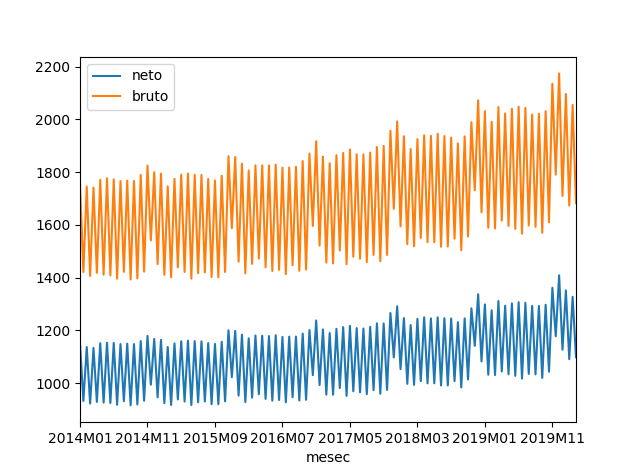
\includegraphics[width=\linewidth]{img/plt_pandas1.png}
    \caption{Črtni graf nad celotno tabelo.}
    \label{img:plt_pandas1}
\end{figure}
Problem dobljenega grafa je, da z isto linijo prikazuje javni in zasebni sektor skupaj. Sektorja moramo torej ločiti. To lahko naredimo kar s filtriranjem:
\begin{lstlisting}[language=python]
df_javni= df[df['sektor']=='Javni sektor'] 
df_zasebni = df[df['sektor']=='Zasebni sektor']
\end{lstlisting}
Zdaj izrišemo oba sektorja. Če ju hočemo narisati na skupnem grafu, oziroma isti osi \angl{axis}, moramo to eksplicitno podati. Najprej pridobimo trenutno os preko funkcije \texttt{gca}:
\begin{lstlisting}[language=python]
ax = plt.gca()
\end{lstlisting}
Potem os podamo pri risanju, skupaj z ostalimi argumenti. Graf lahko dopolnimo še z legendo, oznakami itd.
\begin{lstlisting}[language=python]
df_javni.plot(x='mesec',
              y=['neto','bruto'],
              ax = ax)
df_zasebni.plot(x='mesec',
                y=['neto','bruto'],
                ax = ax)
plt.legend(['Javni sektor (neto)',
          'Javni sektor (bruto)',
          'Zasebni sektor (neto)',
          'Zasebni sektor (bruto)'])
plt.ylabel('Znesek [EUR]')
plt.show()
\end{lstlisting}
Tako dobljen graf prikazuje slika \ref{img:plt_pandas2}.
\begin{figure}
    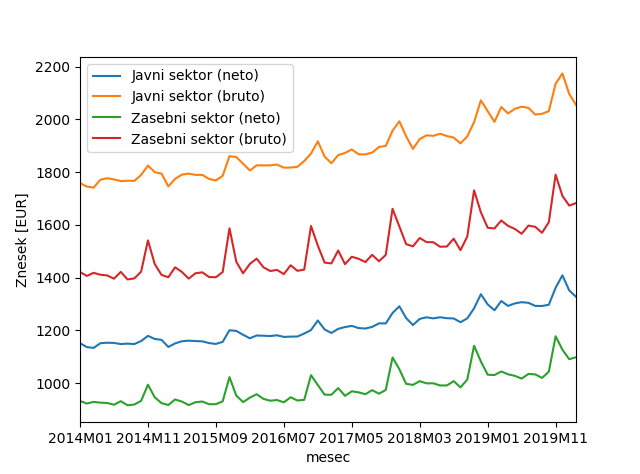
\includegraphics[width=\linewidth]{img/plt_pandas2.png}
    \caption{Črtni graf z ločenim izrisom za javni in zasebni sektor.}
    \label{img:plt_pandas2}
\end{figure}
Graf bi lahko na enostaven način spremenili v kakšen drug tip, tako da bi nastavili izbirni argument \texttt{kind} na kakšno drugo vrednost, npr. \texttt{'bar'} za stolpčni diagram ali pa \texttt{'box'} za izris s kvartili.

Graf bi lahko narisali tudi tako, da bi podatke iz strukture \texttt{dataframe} pretvorili npr. v strukturo \texttt{ndarray} z uporabo metode \texttt{values} (metoda \texttt{values} zavrže imena stolpcev in kot matriko tipa \texttt{ndarray} vrne vsebino tabele). Do matrike bruto in neto plač javnega in zasebnega sektorja, bi lahko npr. prišli takole:
\begin{lstlisting}[language=python]
>>> J = df_javni[['bruto','neto']].values
>>> Z = df_zasebni[['bruto','neto']].values
\end{lstlisting}
Naenkrat lahko narišemo več grafov tudi tako, da funkciji \texttt{plot} (ne metodi) podamo kar matriko. Funkcija bo za vsak stolpec matrike izrisala svoj graf.
\begin{lstlisting}[language=python]
>>> plt.plot(J)
>>> plt.plot(Z)
>>> plt.show()
\end{lstlisting}

\section{Izvoz podatkov}

Podatke lahko iz tabel \texttt{dataframe} tudi enostavno izvozimo. Če bi npr. želeli podatke za javni sektor izvoziti v datoteko CSV, bi to lahko naredili z uporabo metode \texttt{to\_csv}.
\begin{lstlisting}[language=python]
df_javni.to_csv('place_javni.csv', index=False)
\end{lstlisting}
Opcijski argument \texttt{index} smo nastavili na vrednost \texttt{False}, saj ponavadi stolpca z indeksi ne želimo izvažati (včasih pa). 

Podatke bi lahko izvozili tudi v Excelovo datoteko, in sicer z metodo \texttt{to\_excel}, ki deluje zelo podobno kot metoda za izvoz v datoteke CSV:
\begin{lstlisting}[language=python]
df_javni.to_excel('place_javni.xlsx', index=False)
\end{lstlisting}
Na podoben način lahko Excelovo datoteko tudi uvozimo. Tokrat uporabimo funkcijo \texttt{read\_excel}:
\begin{lstlisting}[language=python]
df_javni2 = pd.read_excel('place_javni.xlsx')
\end{lstlisting}
